\addcontentsline{toc}{chapter}{Measurement Data} 
\label{protocol}

% \thispagestyle{empty}

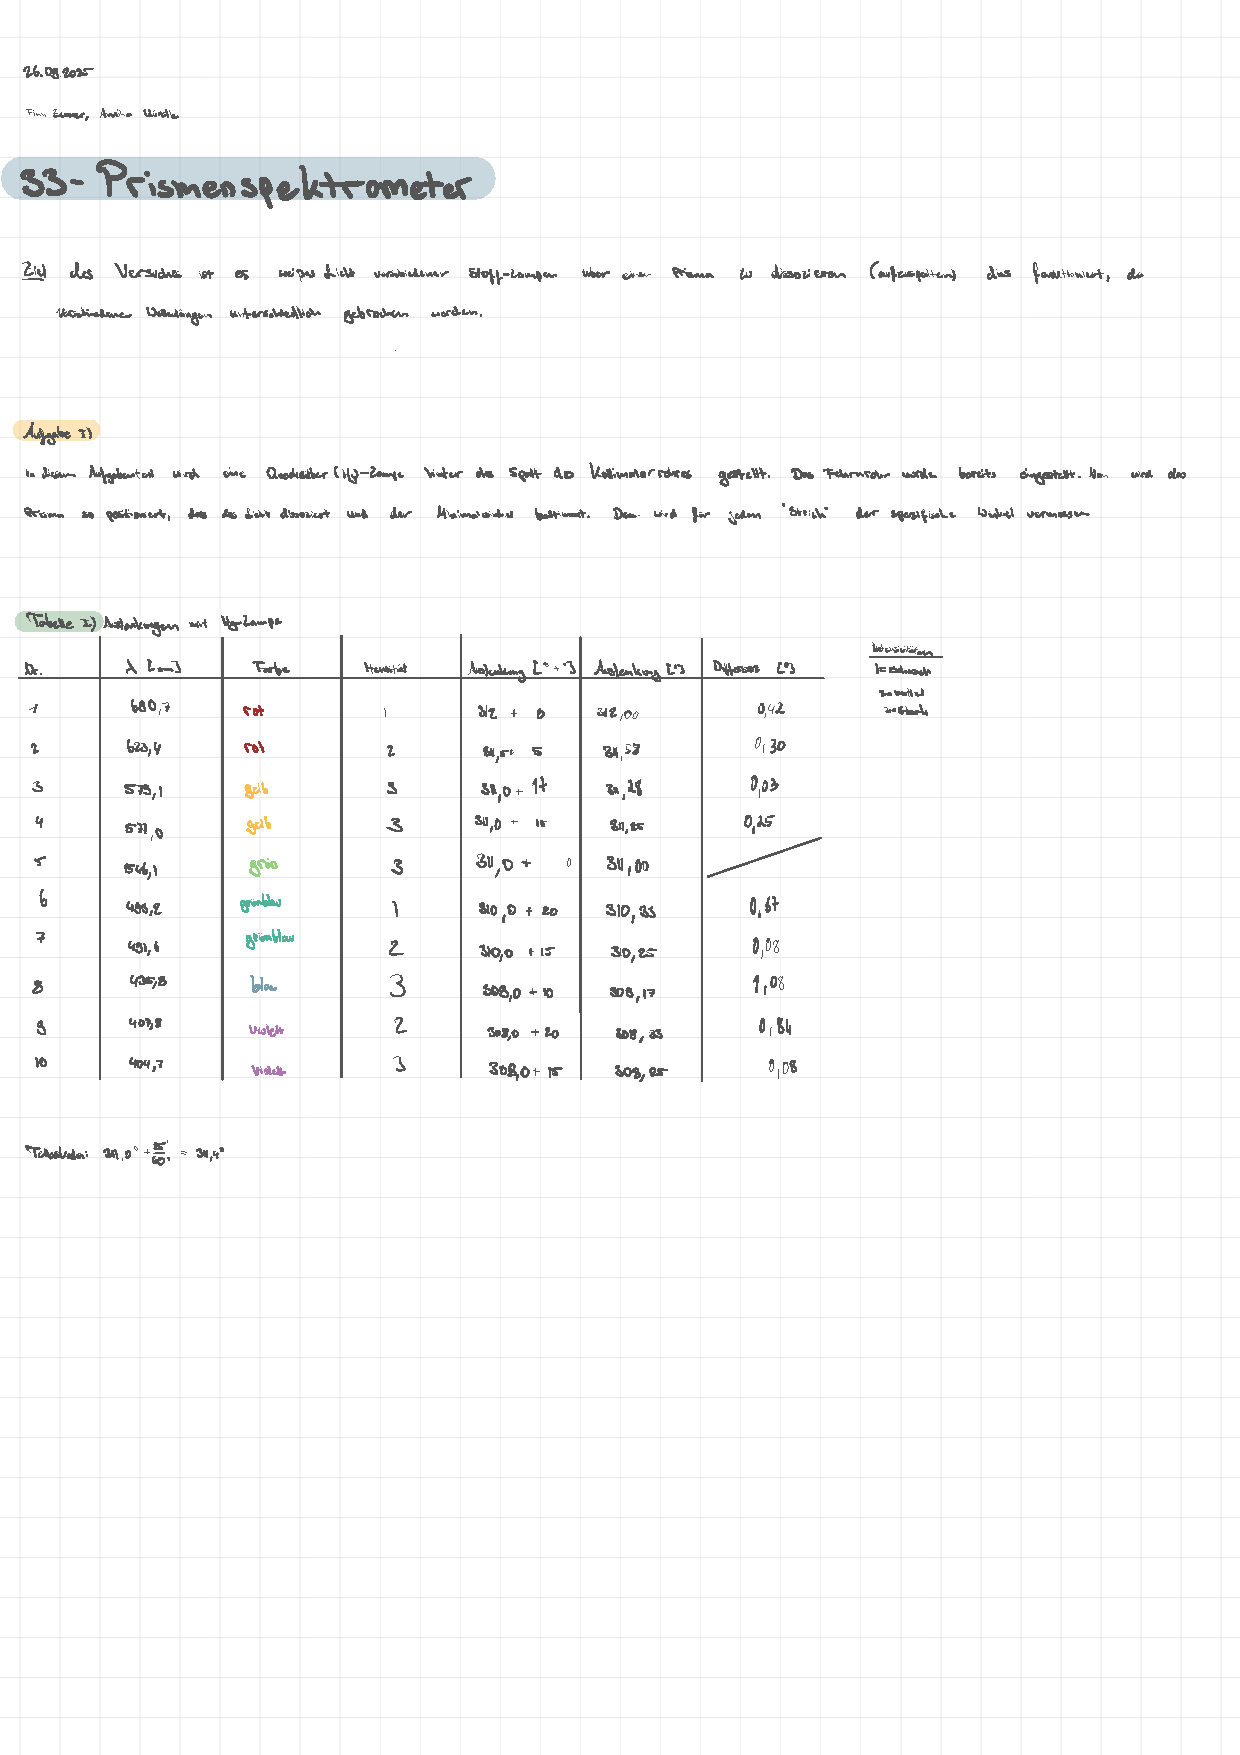
\includepdf[
  pages=1-3,               
  pagecommand={\thispagestyle{empty}} 
]{Protokolle/\versuchsnummer/Chapter/Messprotokoll.pdf}

\addcontentsline{lot}{table}{\protect\numberline{\thechapter.1} Materialeigenschaften}
\addcontentsline{lot}{table}{\protect\numberline{\thechapter.2} Messreihe des Wasserkalorimeters zur Bestimmung des Wasserwertes}
\addcontentsline{lot}{table}{\protect\numberline{\thechapter.3} Messreihe im Wasserkalorimeters Aluminium}
\addcontentsline{lot}{table}{\protect\numberline{\thechapter.4} Messreihe im Wasserkalorimeters Blei}
\addcontentsline{lot}{table}{\protect\numberline{\thechapter.5} Messreihe im Wasserkalorimeters Graphit}
\addcontentsline{lot}{table}{\protect\numberline{\thechapter.5} Messreihe der Körper im Flüssigstickstoff}
